\begin{frame}
	\myheading {Module 3.2: A typical Supervised Machine Learning Setup}
\end{frame}
\begin{frame}
	\begin{columns}
		\column{0.4\textwidth}
		\begin{overlayarea}{\textwidth}{\textheight}
			\vspace{+0.2in}
			\begin{center}
				\textbf{Sigmoid (logistic) Neuron}
				\begin{tikzpicture}
	\node (input0) at (8,-0.1)  {$x_{1}$};
	\node (input1) at (9,-0.1)  {$x_{2}$};
	\node (input2) at (10,-0.1)  {$..$};
	\node (input3) at (11,-0.1)  {$..$};
	\node (input4) at (12,-0.1)  {$x_{n}$};
	\node (input5) at (7,-0.1)  {$x_{0}=1$};

	\node [hidden_neuron] (neuron1) at (10,2)  {};


	\node (output0)  at (10,3.5) {$y$};

	\draw [->] (input0) -- (neuron1);
	\draw [->] (input1) -- (neuron1);
	\draw [->] (input2) -- (neuron1);
	\draw [->] (input3) -- (neuron1);
	\draw [->] (input4) -- (neuron1);
	\draw [->] (input5) -- (neuron1);

	\draw [->] (neuron1) -- (output0);

	\node (formula)[scale=.8] at (8.4,0.6) {$w_{1}$};
	\node (formula)[scale=.8] at (9.1,0.6) {$w_{2}$};
	\node (formula)[scale=.8] at (9.8,0.6) {$..$};
	\node (formula)[scale=.8] at (10.4,0.6) {$..$};
	\node (formula)[scale=.8] at (11.1,0.6) {$w_{n}$};
	\node (formula)[scale=.8] at (7.2,0.6) {$w_{0} = -\theta$};

\end{tikzpicture}

			\end{center}
		\end{overlayarea}
		\column{0.6\textwidth}
		\begin{overlayarea}{\textwidth}{\textheight}
			\begin{itemize}\justifying
				\item<1-> What next ?
				\item<2-> Well, just as we had an algorithm for learning the weights of a perceptron, we also need a way of learning the weights of a sigmoid neuron
				\item<3-> Before we see such an algorithm we will revisit the concept of \textbf{error}
			\end{itemize}
		\end{overlayarea}
	\end{columns}
\end{frame}


\begin{frame}
	\begin{columns}
		\column{0.3\textwidth}
		\begin{overlayarea}{\textwidth}{\textheight}
			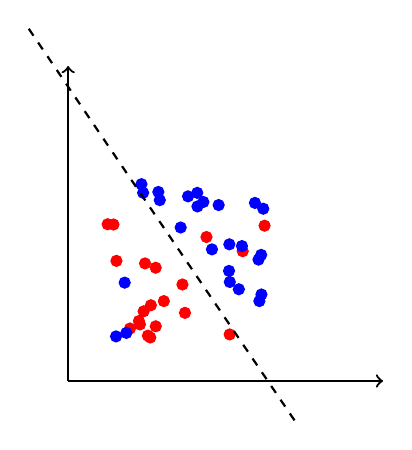
\begin{tikzpicture}
	\filldraw[red] (1.717248,1.148263) circle (2pt);%--
	\filldraw[blue] (1.022337,1.844630) circle (2pt);
	\filldraw[blue] (0.929218,1.449012) circle (2pt);
	\filldraw[red] (1.256599,1.328157) circle (2pt);%--
	\filldraw[blue] (1.917421,1.041134) circle (2pt);
	\filldraw[blue] (1.552910,0.757361) circle (2pt);
	\filldraw[red] (0.476688,0.993158) circle (2pt);
	\filldraw[blue] (1.139669,1.889055) circle (2pt);
	\filldraw[red] (1.994183,1.472244) circle (2pt);%--
	\filldraw[red] (0.611827,0.938297) circle (2pt);
	\filldraw[blue] (1.954791,0.598560) circle (2pt);
	\filldraw[red] (0.113127,1.025315) circle (2pt);
	\filldraw[blue] (1.547272,1.235639) circle (2pt);
	\filldraw[blue] (1.667688,0.664851) circle (2pt);
	\filldraw[blue] (0.108270,0.066074) circle (2pt);%--
	\filldraw[red] (1.551238,0.091185) circle (2pt);
	\filldraw[red] (0.550644,0.461861) circle (2pt);
	\filldraw[blue] (1.326191,1.171462) circle (2pt);
	\filldraw[red] (0.285269,0.166320) circle (2pt);
	\filldraw[blue] (0.645487,1.900755) circle (2pt);
	\filldraw[red] (0.715271,0.514446) circle (2pt);
	\filldraw[blue] (0.239037,0.110620) circle (2pt);%--
	\filldraw[blue] (1.707163,1.213513) circle (2pt);
	\filldraw[blue] (0.663682,1.796715) circle (2pt);
	\filldraw[red] (0.512817,0.075660) circle (2pt);
	\filldraw[blue] (1.542905,0.897760) circle (2pt);
	\filldraw[blue] (1.928409,0.514645) circle (2pt);
	\filldraw[blue] (0.430763,1.999726) circle (2pt);
	\filldraw[red] (0.411993,0.218422) circle (2pt);
	\filldraw[red] (0.951387,0.725352) circle (2pt);
	\filldraw[red] (0.001601,1.490619) circle (2pt);
	\filldraw[red] (0.983530,0.364934) circle (2pt);
	\filldraw[red] (0.612532,0.194346) circle (2pt);
	\filldraw[blue] (1.217355,1.773029) circle (2pt);
	\filldraw[red] (0.398657,0.261244) circle (2pt);
	\filldraw[blue] (0.452156,1.890002) circle (2pt);
	\filldraw[red] (0.458527,0.384611) circle (2pt);
	\filldraw[blue] (1.977895,1.687690) circle (2pt);
	\filldraw[blue] (0.217980,0.748811) circle (2pt);%--
	\filldraw[red] (0.075486,1.486788) circle (2pt);
	\filldraw[blue] (1.872187,1.761516) circle (2pt);
	\filldraw[blue] (1.142016,1.716686) circle (2pt);
	\filldraw[blue] (1.411278,1.734101) circle (2pt);
	\filldraw[blue] (1.951329,1.101424) circle (2pt);
	\filldraw[red] (0.543241,0.052208) circle (2pt);

	\draw[thick,->] (-0.5,-0.5) -- (3.5,-0.5);
	\draw[thick,->] (-0.5,-0.5) -- (-0.5,3.5);

	\onslide<4->{\draw[thick,dashed] (2.374856,-1) -- (-1,3.972960);}
\end{tikzpicture}

		\end{overlayarea}
		\column{0.7\textwidth}
		\begin{overlayarea}{\textwidth}{\textheight}
			\begin{itemize}\justifying
				\item<1-> Earlier we mentioned that a single perceptron cannot deal with this data because it is not linearly separable
				\item<2-> What does ``cannot deal with'' mean?
				\item<3-> What would happen if we use a perceptron model to classify this data ?
				\item<4-> We would probably end up with a line like this ...
				\item<5-> This line doesn't seem to be too bad
				\item<6-> Sure, it misclassifies 3 blue points and 3 red points but we could live with this error in \textbf{most} real world applications
				\item<7-> From now on, we will accept that it is hard to drive the error to 0 in most cases and will instead aim to reach the minimum possible error
			\end{itemize}
		\end{overlayarea}
	\end{columns}
\end{frame}


\begin{frame}
	This brings us to a typical machine learning setup which has the following components...
	\begin{itemize}\justifying
		\item<2-> \textbf{Data:} $\{x_i, y_i\}_{i=1}^{n}$
		\item<3-> \textbf{Model:} Our approximation of the relation between $\mathbf{x}$ and $y$. For example,
		      \onslide<4->{
			      \begin{align*}
				      \onslide<4->{\hat{y}         & = \frac{1}{1 + e^{-\mathbf{(W^T x)}}}} \\
				      \onslide<5->{or\quad \hat{y} & = \mathbf{W^Tx}}                     \\
				      \onslide<6->{or\quad \hat{y} & = \mathbf{x^TWx}}
			      \end{align*}
		      }
		      \onslide<7->{or just about any function}
		\item<8-> \textbf{Parameters:} In all the above cases, $\mathbf{W}$ is a parameter which needs to be learned from the data
		\item<9-> \textbf{Learning algorithm:} An algorithm for learning the parameters ($\mathbf{W}$) of the model (for example, perceptron learning algorithm, gradient descent, etc.)
		\item<10-> \textbf{Objective/Loss/Error function:} To guide the learning algorithm \onslide<11->{- the learning algorithm should aim to minimize the loss function}
	\end{itemize}
\end{frame}

\begin{frame}
	As an illustration, consider our movie example
	\begin{itemize}\justifying
		\item<2-> \textbf{Data:} $\{x_i = movie, y_i = like/dislike\}_{i=1}^{n}$
		\item<3-> \textbf{Model:} Our approximation of the relation between $\mathbf{x}$ and $y$ (the probability of liking a movie).
		      \onslide<4->{
			      \begin{align*}
				      \onslide<4->{\hat{y} & = \frac{1}{1 + e^{\mathbf{-(W^T x)}}}} \\
			      \end{align*}
		      }
		      \vspace{-0.3in}
		\item<5-> \textbf{Parameter:} $\mathbf{W}$
		\item<6-> \textbf{Learning algorithm:} Gradient Descent [we will see soon]
		\item<7-> \textbf{Objective/Loss/Error function:} \onslide<8->{One possibility is
			      %\vspace{-0.1in}
			      \begin{align*}
				      \onslide<8->{\mathscr{L}(\mathbf{W}) = \sum_{i=1}^{n} (\hat{y}_i - y_i)^2} \\
			      \end{align*}
		      }
		      %\vspace{-0.1in}
		      \onslide<9->{The learning algorithm should aim to find a $\mathbf{W}$ which minimizes the above function (squared error between $y$ and $\hat{y}$)}
	\end{itemize}
\end{frame}
